\documentclass[../dissertation.tex]{subfiles}

\begin{document}

\section{Experiment 8 - Vertical Scaling On Car Platform}
\label{experiment8-vertical-scaling}

\paragraph{Introduction} Prior experiments have been completed using what was called `bare' Raspberry Pi hosts. This refers to the fact that they are off-the-shelf Raspberry Pis with no peripherals or modifications, using standard mains power. However, the test platform described in Section \ref{background-robot-config} represents a more realistic scenario, utilising a more unreliable power source (a battery), and several peripherals (such as a video camera). These differences in the host configuration are not expected to affect performance of the vertical scaling limits in the host (since the car platform utilises the same model of Raspberry Pi) - however, this must be experimentally confirmed.

\paragraph{Objective} This experiment aims to verify the results of experiment 7 (Section \ref{experiment7-vertical-scaling}) on a real robot platform - namely the robot kit cars described in Section \ref{background-robot-config}.

\paragraph{Hypothesis} The expected outcome of the experiment is that the conclusions of Section \ref{background-robot-config} will hold true, as those prior experiments were run a test platform that is fundamentally similar to the robot car platform. If a performance drop were to be seen, it is expected that this would be due to the different power supply mechanisms between the bare Raspberry Pis and the robot car kit platform (mains power and batteries, respectively).

\paragraph{Materials and Methodology} As this experiment is effectively a re-run of Experiment 7 (as presented in Section \ref{experiment7-vertical-scaling}), this experiment has the same methodology as Experiment 7, but conducted on the robot car platform. This presents some new challenges in the execution of the experiment. Due to the battery power supply, the entire experiment (3 runs at 3 message frequencies with 8 different node counts) can not be run in a single battery lifetime. A single charge lasts long enough for 1.5 runs, however in order to reduce likelihood of inconsistent data it was decided to conduct the experiment 1 run at a time, with a battery charge conducted between runs - thus the experiment had to be executed over a number of days.

\paragraph{Results and Discussion} Figure \ref{exp8-all-freqs-averages} shows a similar graph as Figure \ref{exp7-further-all-freqs-averages}, but with data acquired from 3 runs on the robot car kit platform. It shows that the results gathered in Experiment 7 were valid on the robot car kit platform, as we see spikes in the message latency at the same node counts as in the previous experiment on the bare Raspberry Pis. Note that 128 node, and 256 node counts were skipped for 10Hz, and 64, 128, and 256 were skipped for 20Hz due to the extremely long time it takes those setups to conclude their runs (on the scale of several hours) - and the robot cars would run out of battery before all sending/receiving nodes can finish. However, the node counts that have been run demonstrate that the performance bottlenecks occur at the same node counts.

\begin{figure}[H]
\centering
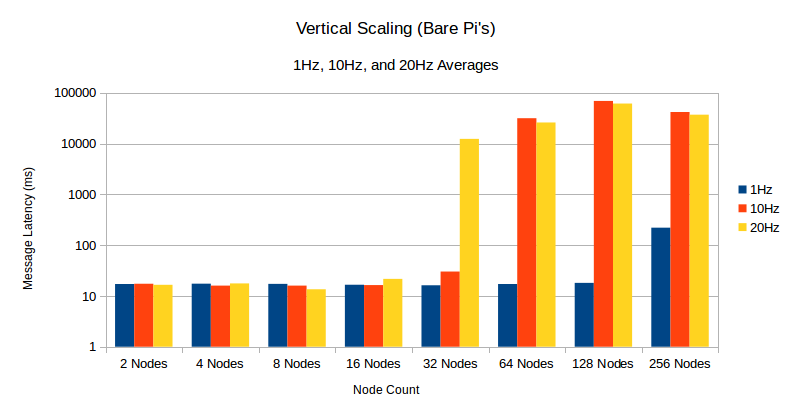
\includegraphics[width=\textwidth]{images/experiment9/vertical_scaling_all_freqs_log_avg_msg_latency.png}
\caption{Experiment 8 - Logarithmic Average Message Latency, All Frequencies, All Node Counts}
\label{exp8-all-freqs-averages}
\end{figure}

\textit{Therefore we can conclude that CSLV as presented in Section \ref{experiment7-vertical-scaling} is a concern for real ROS systems, and that for this specific set-up (utilising Raspberry Pi 3 Model Bs on WiFi) the limit is approximately between (4.25 * 10 * 16 =) 680kB/s and (4.25 * 20 * 16 =) 1360kB/s depending on exact message latency tolerance.}

\end{document}
